\chapter{Schémas aux différences}

\section{Opérateurs aux différences en dimension 1}

\subsection{Notations}
\label{sec:notation_1D}

On considère $\Omega = [a,b]$, $a<b$, un intervalle de $\mathbb{R}$ de longueur $L=b-a$. Nous utilisons les lettres latines pour noter les fonctions continues : $f(x)$, $u(x)$, ... $x \in \Omega$ à valeur complexe. Pour $u$ et $v$, des fonctions définies sur $\Omega$, le produit scalaire $L^2 ( \Omega )$ est défini par
\begin{equation}
(u,v) = \gint_{\Omega} u(x) \bar{v}(x) dx = \gint_{a}^b u(x) \bar{v}(x) dx.
\end{equation}
Pour $u$ et $v$ à valeurs réelles, on a
\begin{equation}
(u,v) = \gint_{a}^b u(x) v(x) dx.
\end{equation}
La norme sur $L^2(\Omega)$ est donnée par :
\begin{equation}
\| u \|_{L^2(\Omega)} = \sqrt{(u,u)}
\end{equation}
Pour $u \in \mathcal
C(\bar{\Omega}) \cap L^{\infty}(\Omega)$, on note
\begin{equation}
\| u \|_{\infty} = \sup_{x\in\Omega} |u(x)|.
\end{equation}
Une fonction $u : x \in \mathbb{R} \mapsto u(x) \in \mathbb{R}$ est \textit{périodique} de période $L$ si 
\begin{equation}
u(x+L) = u(x) \text{, } \forall x \in \mathbb{R}.
\end{equation}
En particulier, on a $u(a)=u(b)$.

On considère une grille régulière sur $\Omega$ constituée de $N \geq 1$ points :
\begin{equation}
a=x_0 < x_1 < \ldots < x_{N-1} < x_N = b,
\end{equation}
où les valeurs $x_i$ sont définies par :
\begin{equation}
x_i = a + ih\text{, } i = 0,1, \ldots,N \text{ et } h = \dfrac{b-a}{N} \text{ le pas d'espace}. 
\end{equation}

\begin{figure}[htbp]
\begin{center}
\begin{tikzpicture}[scale=1.8]
	\draw [>=stealth, <->] (-2,0.2) -- (-1,.2) ;
	\draw (-1.5,.3) node[above] {$h$} ;
	\draw (-3,0) -- (3,0) ;
	\draw (-3,0) node {$\times$} ;
	\draw (-3,-.2) node[below] {$x_0=a$} ;
	\draw (-2,0) node {$\bullet$} ;
	\draw (-2,-.2) node[below] {$x_1$} ;
	\draw (-1,0) node {$\bullet$} ;
	\draw (-1,-.2) node[below] {$x_2$} ;
	\draw (0,-.2) node[below] {$\ldots$} ;
	\draw (1,0) node {$\bullet$} ;
	\draw (1,-.2) node[below] {$x_{N-2}$} ;
	\draw (2,0) node {$\bullet$} ;
	\draw (2,-.2) node[below] {$x_{N-1}$} ;
	\draw (3,0) node {$\times$} ;
	\draw (3,-.2) node[below] {$x_N =b$} ;
\end{tikzpicture}
\end{center}
\caption{Grille en dimension 1. Les symboles $\times$ désignent les points de bords, les symboles $\bullet$ désignent les points intérieurs de la grille.}
\label{fig:maillage1D}
\end{figure}

Les points $x_0=a$ et $x_N = a + L = b$ sont les points de bord du domaine et les points $(x_j)_{1 \leq j \leq N-1}$ désignent les points intérieurs. 

Nous distinguons trois types de données aux points de grille $x_j$, $0 \leq j \leq N$ :
\begin{enumerate}
\item Une \textit{fonction de grille} est une fonction définie uniquement aux points $(x_j)_{0 \leq j \leq N}$. Les fonctions de grilles sont notées en fonte gothique : $\mathfrak{u}$, $\mathfrak{v}$, ... 
On note
\begin{equation}
\mathfrak{u} = (\mathfrak{u}(x_0), \mathfrak{u}(x_1), \mathfrak{u}(x_2), ... , \mathfrak{u}(x_N)).
\end{equation}
De plus, $l^2_h$ désigne l'espace des fonctions de grille, $h>0$ fixé.
On munit cet espace du produit scalaire et de la norme associée :
\begin{equation}
(\mathfrak{u},\mathfrak{v})_h = h \gsum_{j=0}^N \mathfrak{u}(x_j) \mathfrak{v}(x_j) \text{,  } |\mathfrak{u}|_h^2 = h \gsum_{j=0}^N \mathfrak{u}(x_j)^2.
\end{equation}
On définit aussi la norme infinie pour les fonctions de grille :
\begin{equation}
\| \mathfrak{u} \|_{\infty} = \max_{0\leq j \leq N} |\mathfrak{u}(x_j)|.
\end{equation}
On notera 
\begin{equation}
\mathfrak{u}_j = \mathfrak{u}(x_j) \text{ pour tout } 0\leq j \leq N.  
\end{equation}

On note $l^2_{h,per}$ l'espace des fonctions de grilles périodiques. Si $\mathfrak{u} \in l^2_{h,per}$ alors $\mathfrak{u}(x_0) = \mathfrak{u}(x_N)$ et on a
\begin{equation}
\mathfrak{u}=(\mathfrak{u}(x_0), \mathfrak{u}(x_1), ..., \mathfrak{u}(x_{N-1})).
\end{equation}
Le produit scalaire et la norme associée dans $l^2_{h,per}$ sont
\begin{equation}
(\mathfrak{u},\mathfrak{v})_{h,per} = h \gsum_{j=1}^N \mathfrak{u}(x_j) \mathfrak{v}(x_j) \text{,  } |\mathfrak{u}|_h^2 = h \gsum_{j=1}^N \mathfrak{u}(x_j)^2 \text{ avec} \mathfrak{u}, \mathfrak{v} \in l^2_{h,per}.
\end{equation}
La norme infinie dans $l^2_{h,per}$ est
\begin{equation}
\| \mathfrak{u} \|_{\infty} = \max_{1\leq j \leq N} |\mathfrak{u}(x_j)|.
\end{equation}



\item Les lettres latines capitales désignent les vecteurs de $\mathbb{R}^{N+1}$ et les matrices de $\mathbb{M}_{N+1}(\mathbb{R})$. Par exemple, soit le vecteur $U \in \mathbb{R}^{N+1}$ des composantes de $\mathfrak{u} \in l^2_h$ :
\begin{equation}
U = \begin{bmatrix}
\mathfrak{u}_0 \\ \mathfrak{u}_1 \\ \vdots \\ \mathfrak{u}_N
\end{bmatrix} =
\begin{bmatrix}
\mathfrak{u}(x_0) \\ \mathfrak{u}(x_1) \\ \vdots \\ \mathfrak{u}(x_N)
\end{bmatrix}
\end{equation}
La norme euclidienne sur $\mathbb{R}^{N+1}$ est notée $|U|$. Elle induit une norme pour les matrices $A \in \mathbb{M}_{N+1}(\mathbb{R})$ définie par
\begin{equation}
|A|_2 = \sup_{U \neq 0} \dfrac{|AU|}{|U|}.
\end{equation}
Si $A$ est symétrique alors :
\begin{equation}
|A|_2 = \rho(A) := \max \left\lbrace |\lambda| \text{ tels que } \lambda \in \Sp (A) \right\rbrace.
\end{equation}
$\rho(A)$ est nommé \textit{rayon spectrale} de $A$.
La norme infinie de $U$ est donnée par :
\begin{equation}
|U|_{\infty} = \max_{1 \leq j \leq N+1} |U_j|.
\end{equation}
La norme sur $\mathbb{M}_{N+1}(\mathbb{R})$ subordonnée à $|\cdot|_{\infty}$ est
\begin{equation}
|A|_{\infty} = \sup_{U \neq 0} \dfrac{|AU|_{\infty}}{|U|_{\infty}} = \max_{1 \leq i \leq N+1} \gsum_{j=1}^{N+1} |A_{i,j}|.
\end{equation}



\item Soit $u: x \in \Omega \mapsto u(x)$, on définit la \textit{fonction de grille} $u^*$ associée à $u$ par :
\begin{equation}
u^*_j = u^*(x_j) \text{ pour } 0 \leq j \leq N.
\end{equation}
$u^*$ est donc la restriction de $u$ aux points de la grille. Si $u$ est une fonction périodique, alors $u^*$ est définit par
\begin{equation}
u^*_j = u^*(x_j) \text{ pour } 1 \leq j \leq N.
\end{equation}
\end{enumerate}

Nous distinguons $l^2_h$, l'espace des fonctions de grilles, de $\mathbb{R}^{N+1}$ même si ces deux espaces sont isomorphes.

Cette distinction permet de faire une claire différences entre :
\begin{itemize}
\item les opérateurs aux différences finies, qui agissent sur les fonctions de grilles,
\item les matrices, qui agissent sur les vecteurs.
\end{itemize}
Les fonctions de grilles contiennent toutes les échelles nécessaires dans le contexte physique alors que les vecteurs sont sans dimension. De plus, le raisonnement au niveau discret est plus naturel avec les fonctions de grilles. Il s'effectue d'une façon abstraite à l'aide d'opérateurs aux différences. En revanche, le codage est effectuée dans le cadre de l'algèbre linéaire.

Si $u : x \in \Omega \mapsto u(x) \in \mathbb{R}$est une fonction régulière telle que $u(a) = u(b) = 0$ alors $(\partial_x u)^*$ désigne la restriction à la grille de la fonction $\partial_x u$ associée à la dérivée première de $u$. On peut approcher cette donnée à l'aide de $\mathfrak{u}_x$ obtenue grâce à l'opérateur $\delta_x$ agissant sur les fonctions de grilles et donné par
\begin{equation}
\mathfrak{u}_{x,j} = \delta_x u^*(x_j) = \dfrac{u(x_{j+1}) - u(x_{j-1})}{2h}.
\end{equation}
En effet, par développement de Taylor, on a 
\begin{equation}
u(x_j+h) = u(x_j) + h \partial_x u(x_j) + \dfrac{h^2}{2} \partial_x^2 u(x_j) + \dfrac{h^3}{6} \partial_x^3 u(\xi) \text{ avec } \xi \in [x_j, x_j+h].
\end{equation}
De la même manière, en $x_j-h$, on a 
\begin{equation}
u(x_j-h) = u(x_j) - h \partial_x u(x_j) + \dfrac{h^2}{2} \partial_x^2 u(x_j) - \dfrac{h^3}{6} \partial_x^3 u(\eta) \text{ avec } \eta \in [x_j-h, x_j].
\end{equation}
Soit $0 \leq j \leq N$, alors
\begin{align*}
\delta_x u^*(x_j) & = \dfrac{u(x_{j+1}) - u(x_{j-1})}{2h}\\
                  & = \dfrac{1}{2h} \left[ 2h \partial_x u(x_j) + \dfrac{h^3}{6} \partial_x^3 u(\xi) + \dfrac{h^3}{6} \partial_x^3 u(\eta) \right]\\
                  & = \partial_x u(x_j) + \dfrac{h^2}{2} \left[ \dfrac{1}{6} \partial_x^3 u(\xi) + \dfrac{1}{6} \partial_x^3 u(\eta) \right] \\
                  & = \partial_x u(x_j) + \dfrac{h^2}{6} \partial_x^3 u(\gamma) \text{ avec } \gamma \in ]x_j-h , x_j+h[ \text{ par théorème des valeurs intermédiaires.}
\end{align*}
L'erreur de troncature est une fonction de grille définie en chaque point du $x_j$ par
\begin{align*}
\mathfrak{t}(x_j) & = \delta_x u^*(x_j) - \delta_x u^*(x_j)\\
                  & = \dfrac{h^2}{6} \partial_x^3 u(\gamma) \text{ avec } \gamma \in ]x_j-h , x_j+h[.
\end{align*}

















\subsection{Opérateur de translation périodique}
Les notations employées sont celles de la partie \ref{sec:notation_1D} dans le contexte périodique avec $a=0$ et $b=L$. Soit $\mathfrak{u} \in l^2_{h,per}$.

\begin{definition}
L'opérateur $\tau_p$, $p \in \mathbb{Z}$, est définit, pour $\mathfrak{u}$ une fonction de grille périodique, pour tout $1 \leq j \leq N$ par
\begin{equation}
(\tau_p \mathfrak{u})_j = \mathfrak{u}_{j+p}.
\end{equation}
\end{definition}
L'opérateur linéaire $\tau_p$ agit sur les fonctions périodiques $u : \mathbb{R} \mapsto u(x) \in \mathbb{R}$ par :
\begin{equation}
\tau_p u(x_j) = (\tau_p u^*)_j = u^*_{j+p} = u(x_{j+p}).
\end{equation}
En particulier, lorsque $p=1$, on note $\tau$ l'\textit{opérateur de translation à droite} :
\begin{equation}
\tau = \tau_{1}
\end{equation}
de plus, il est clair que l'on a
\begin{equation}
\begin{array}{rcl}
\tau^0 & = & id\\
\tau^p & = & \underbrace{\tau \circ \tau \circ \tau \circ \cdots \circ \tau}_{p \text{ fois.}}
\end{array}
\end{equation}
L'égalité suivante est vérifiée :
\begin{equation}
\tau^p = \tau_p
\end{equation}
En particulier, on a $\tau^N = \tau_N = id$, donc $\tau$ est inversible et
\begin{equation}
\tau^{-1} = \tau^{N-1}.
\end{equation}
L'analyse des opérateurs périodiques repose sur la diagonalisation de $\tau$. C'est l'objet de la proposition suivante.

\begin{proposition}
les valeurs propres de $\tau$ sont les racines de l'unité $\omega^k \in \mathbb{C}$ avec
\begin{equation}
\omega = \exp \left[ i \dfrac{2 \pi}{N} \right].
\end{equation}

Chaque valeur propre $\omega^k$ est associée à une fonction propre $\mathfrak{u}^k$ périodiques :
\begin{equation}
\mathfrak{u}_j^k = \dfrac{1}{\sqrt{N}}  \exp \left[ i j \dfrac{2 \pi k}{N} \right]
\label{eq:vecteurpropre_tau}
\end{equation}
avec $-\frac{N}{2}+1 \leq k \leq \frac{N}{2}$.
\label{prop:eigenvaluevector_tau}
\end{proposition}

\begin{proof}
Soit $j$ et $k$ tels que $1 \leq j \leq N$ et $-\frac{N}{2}+1 \leq k \leq \frac{N}{2}$. Alors
\begin{equation}
(\tau \mathfrak{u}^k)_j = \mathfrak{u}^k_{j+1}  = \exp \left[ i (j+1) \dfrac{2 \pi k}{N} \right] = \exp \left[ i j \dfrac{2 \pi k}{N} \right] \exp \left[ i \dfrac{2 \pi k}{N} \right]  = \omega^k \mathfrak{u}_j^k
\end{equation}
d'où le résultat.
\end{proof}
Connaissant les valeurs et fonctions propres de $\tau$, on déduit en déduit la diagonalisation de $\tau$.

\begin{corollaire}
L'opérateur $\tau$ est diagonalisable et 
\begin{equation}
\tau = \gsum_{k = -N/2+1}^{N/2} \omega^k \mathfrak{u}^k
\end{equation}
où les fonctions propres $\mathfrak{u}^k$ et les valeurs propres $\omega^k$ sont données dans la proposition \ref{prop:eigenvaluevector_tau}
\end{corollaire}
Soit $P \in \mathbb{C}[X]$ un polynôme alors les valeurs propres et fonctions propres de $P(\tau)$ sont connues.

\begin{proposition}
Les fonctions propres de $P(\tau)$ sont les fonctions de grilles $\mathfrak{u}^k$.
Chaque fonction propre est associé à la valeur propre $P(\omega^k)$ avec $-N/2+1 \leq k \leq N/2$.
\label{prop:eigen_tau}
\end{proposition}

\begin{proof}
$P$ est un polynôme de $\mathbb{C}[X]$ donc il existe un nombre finis d'éléments de $\mathbb{C}$ notés $a_0$, $a_1$, $a_2$, ... tels que
\begin{equation}
P(X) = \gsum_{n=0} a_n X^n.
\end{equation}
Soient $j$ et $k$ tels que $1 \leq j \leq N$ et $-N/2+1 \leq k \leq N/2$, alors 
\begin{equation}
(P(\tau) \mathfrak{u}^k)_j = \left( \gsum_{n=0} a_n \tau_n \mathfrak{u}^k \right)_j = \gsum_{n=0} a_n \mathfrak{u}^k_{j+n}  = \gsum_{n=0} a_n (\omega^k)^n \mathfrak{u}^k_j = P(\omega^k) \mathfrak{u}^k_j
\end{equation}
d'où le résultat.
\end{proof}

Notons que cette proposition est vraie pour tout opérateur diagonalisable à la place de $\tau$.

L'opérateur de translation $\tau$ agit sur les fonctions de grilles $\mathfrak{u}$. Il est associé à $T \in \mathbb{M}_N \left( \mathbb{R} \right)$ la matrice agissant sur les vecteurs $U$ de $\mathbb{R}^N$.
On définit $\vec_1$ l'opérateur transformant un élément de $l_{h,per}^2$ en un vecteur de $\mathbb{R}^N$ :

\begin{definition}
Soient $\mathfrak{u} \in l^2_{h,per}$ une fonction de grille et $(\mathbf{e}_j)_{1 \leq j \leq N}$ la base canonique de $\mathbb{R}^N$. On définit l'opérateur $\vec_1$ par :
\begin{equation}
\begin{array}{rcl}
\vec_1 : l^2_{h,per} & \rightarrow & \mathbb{R}^N\\
         \mathfrak{u} & \mapsto & \vec_1 ( \mathfrak{u} ) 
\end{array}
\end{equation}
avec 
\begin{equation}
\vec_1 ( \mathfrak{u} ) =\gsum_{j=1}^N \mathfrak{u}_{j-1} \mathbf{e}_j.
\end{equation}
\end{definition}

Il s'agit d'un opérateur transformant directement une fonction de grille $\mathfrak{u} \in l^2_{h,per}$ en un vecteur $U$ de $\mathbb{R}^N$ 
\begin{equation}
U = \vec_1( \mathfrak{u} ) = \begin{bmatrix}
\mathfrak{u}_0\\
\mathfrak{u}_1\\
\vdots\\
\mathfrak{u}_{N-1}\\
\end{bmatrix}
\end{equation}
La matrice $T$ est donnée par

\begin{equation}
T = \begin{bmatrix}
0 & 1 &   &   &   \\ 
  & 0 & 1 & (0) &   \\ 
  &   & \ddots & \ddots &   \\ 
  & (0) &   & 0 & 1 \\ 
1 &   &   &   & 0
\end{bmatrix} 
\end{equation}

La matrice $T$ agit sur un vecteur $U = \begin{bmatrix}
U_0 & U_0 & \cdots & U_{N-1} 
\end{bmatrix}^T \in \mathbb{R}^N $ de telle manière que, pour tout $1 \leq j \leq N$, on a 
\begin{equation}
(TU)_j = U_{j+1}
\end{equation}
C'est à dire
\begin{equation}
\vec_1 ( \tau \mathfrak{u} ) = T \vec_1 ( \mathfrak{u} ). 
\end{equation}
Les propriétés concernant les valeurs propres de $\tau$ sont aussi vérifiées par $T$.

\begin{corollaire}
\begin{itemize}
\item Les valeurs propres de $T$ sont les valeurs $(\omega^k)_{-N/2+1 \leq k \leq N/2}$. 
Chaque valeur propre est associée à un vecteur propre $U^k$ vérifiant :
\begin{equation}
U^k = \vec_1 (\mathfrak{u}^k )
\label{eq:eigenvectorT}
\end{equation}
où $\mathfrak{u}^k$ et $\omega$ sont données dans la proposition \ref{prop:eigenvaluevector_tau}.

\item Si $P \in \mathbb{R}_{N-1}[X]$ alors les valeurs propres de $P(T)$ sont 
\begin{equation}
P(\omega^k)
\end{equation}
chaque valeur propre $P(\omega^k)$ de $T$ est associée au vecteur propre $\vec_1 (\mathfrak{u}^k )$.
\end{itemize}
\label{prop:eigen_P(tau)}
\end{corollaire}

Les vecteurs propres de $T$ forment une base orthonormée de $\mathbb{R}^N$ pour le produit scalaire usuel, en effet
\begin{equation}
(\bar{U^k})^T \cdot U^{k'} = \delta_{k,k'}
\end{equation}
où $\delta_{k,k'}$ désigne le symbole de Kronecker et vaut $1$ si $k=k'$ et $0$ sinon.











\subsection{Transformée de Fourier discrète}

L'espace des fonctions de grille périodique $l^2_{h,per}$ forme un espace vectoriel de dimension $N$. Les vecteurs $(\mathfrak{u}^k)_{-N/2+1 \leq k \leq N/2}$ forment une base orthonormée de cet espace. En effet, soient $-N/2+1 \leq k, k' \leq N/2$, alors 
\begin{equation}
(\mathfrak{u}^k, \mathfrak{u}^{k'})_{h,per} = \delta_{k,k'}.
\end{equation}

Si $\mathfrak{v} \in l^2_{h,per}$, alors il existe $(\hat{\mathfrak{v}}^k )_{-N/2 \leq k \leq N/2}$ tels que 
\begin{equation}
\mathfrak{v} = \gsum_{-N/2+1}^{N/2} \hat{\mathfrak{v}}^k \mathfrak{u}^k
\end{equation}
En effectuant un produit scalaire par $\mathfrak{u}^{k'}$ un vecteur de base, on obtient
\begin{align*}
(\mathfrak{v}, \mathfrak{u}^{k'})_{h,per} & = \gsum_{k=-N/2+1}^{N/2} \hat{\mathfrak{v}}^k (\mathfrak{u}^k, \mathfrak{u}^{k'})_{h,per} \\
		& = \hat{\mathfrak{v}}^{k'}
\end{align*}
Ainsi, les coefficients $\hat{\mathfrak{v}}^{k}$ sont donnés par
\begin{equation}
\hat{\mathfrak{v}}^{k} = (\mathfrak{v}, \mathfrak{u}^{k})_{h,per}.
\end{equation}

De plus, la relation de Parseval est vérifiée.
\begin{proposition}
\textbf{(Relation de Parseval discrète)} Pour tout $\mathfrak{v} \in l^2_{h,per}$, on a 
\begin{equation}
|\mathfrak{v}|_h^2 = \gsum_{k = -N/2+1}^{N/2} |\hat{\mathfrak{v}}^{k}|^2
\end{equation}
\end{proposition}



















\subsection{Opérateurs aux différences discrets}

Soit $L$ un opérateur différentiel. On s'intéresse ici à approcher cet opérateur par $L_h$ et à estimer l'erreur commise via cette approximation.

\begin{definition}
Le couple $(L_h, R_h)$ est consistant avec $L$ à l'ordre $\alpha$ si pour tout $u : \mathbf{x} \in \mathbb{R} \mapsto u(\mathbf{x}) \in \mathbb{R}$ régulière et périodique alors 
\begin{equation}
L_h u^* - R_h (\mathcal{L}(u)^* = \mathcal{O} \left ( h^{\alpha} \right)
\end{equation}
avec $R_h$ un opérateur d'interpolation et $L_h$ un opérateur d'approximation de $\mathcal{L}$.
\end{definition}







Introduisons l'\textit{opérateurs aux différences centré} usuel
\begin{equation}
\delta_x = \dfrac{\tau_1 - \tau_{-1}}{2h}
\end{equation}
Appliqué à la fonction de grille $\mathfrak{u}$, cet opérateur vérifie 
\begin{equation}
\delta_x \mathfrak{u}_i = \dfrac{\mathfrak{u}_{i+1} - \mathfrak{u}_{i-1}}{2h} \text{ pour } 1 \leq i \leq N.
\end{equation}
Il s'agit d'un opérateur permettant d'approcher la dérivée première au sens où

\begin{proposition}
Soit $u: x \in \Omega \mapsto u(x) \in \mathbb{R}$ et $u^*$ la fonction de grille correspondante. Si $u \in \mathcal{C}^3 (\Omega)$ alors 
\begin{equation}
\delta_x u^*_i - u'(x_i) = \dfrac{h^2}{6} u^{(3)}(\alpha_i) \text{ avec } \alpha_i \in [x_{i-1}, x_{i+1}],
\end{equation}
\end{proposition}

\begin{proof}
Comme $u$ est de classe $\mathcal{C}^3$, on considère les développements de Taylor :
\begin{equation}
u(x_i+h) = u(x_i) + h u'(x_i) + \dfrac{h^2}{2} u''(x_i) + \dfrac{h^3}{6} u^{(3)} (\eta_i) \text{ avec } \eta_i \in [x_i, x_{i+1}]
\end{equation}
et celui en $x-h$ :
\begin{equation}
u(x_i-h) = u(x_i) - h u'(x_i) + \dfrac{h^2}{2} u''(x_i) - \dfrac{h^3}{6}u^{(3)}(\xi_i) \text{ avec } \xi_i \in [x_{i-1}, x_{i}]
\end{equation}
Alors par différence, on retrouve la formule souhaitée : 
\begin{equation}
\delta_x u^*_i = u'(x_i) + \dfrac{h^2}{12} \left[ u^{(3)}(\xi_i) + u^{(3)}(\eta_i) \right]  \text{ avec } \xi_i, \eta_i \in [x_{i-1}, x_{i+1}],
\end{equation}
On conclut grâce au théorème des valeurs intermédiaires.
\end{proof}

Ainsi, $\delta_x$ est un opérateur d'approximation de la dérivée première à l'ordre 2. 
















































\subsubsection{Schémas Hermitien}

Dans son article \cite{Lele1991}, S. K. Lele présente une méthode permettant d'approcher la dérivée en un point en ajoutant une partie implicite aux schémas classiques. Définissons l'opérateur de Simpson $\sigma_{x}$ par :

\begin{equation}
\sigma_{x}  = \dfrac{1}{6} \tau_1 + \dfrac{4}{6} id + \dfrac{1}{6}\tau_{-1}
\end{equation}
En particulier, si $\mathfrak{u}$ est une fonction de grille périodique,
\begin{equation}
\sigma_x \mathfrak{u}_j = \dfrac{1}{6} \mathfrak{u}_{j+1} + \dfrac{4}{6} \mathfrak{u}_j + \dfrac{1}{6} \mathfrak{u}_{j-1}
\end{equation}

Les valeurs propres de $\sigma_x$ sont connues.
\begin{proposition}
Les valeurs propres de $\sigma_x$ sont 
\begin{equation}
\mu^k = \dfrac{2}{3} + \dfrac{1}{3} \cos \left( \dfrac{2 \pi k}{N} \right)
\end{equation}
avec $1 \leq k \leq N$. Chaque valeur propre $\mu^k$ est associée à la fonction propre $\mathfrak{u}^k$ donnée en proposition \ref{prop:eigen_tau}.
\label{prop:vp_sigma}
\end{proposition}

\begin{proof}
La proposition \ref{prop:eigen_P(tau)} permet de voir que $\mathfrak{u}^k$ est la fonction propre associée à $\mu^k$ avec 
\begin{equation}
\mu^k = \dfrac{4}{6} + \dfrac{1}{6} \left( \exp \left[ i \dfrac{2 \pi k}{N} \right] + \exp \left[ - i \dfrac{2 \pi k}{N} \right] \right) = \dfrac{2}{3} + \dfrac{1}{3} \cos \left( \dfrac{2 \pi k}{N} \right).
\end{equation}
On a alors $N$ valeurs propres distinctes, d'où le résultat.
\end{proof}
En particulier, on remarque que 
\begin{equation}
\mu^k \neq 0 \text{ pour tout } 1 \leq k \leq N
\end{equation}
donc $\sigma_x$ est inversible.

\begin{corollaire}
L'opérateur $\sigma_x$ est inversible.
\end{corollaire}
De plus, on note que si $u : x \in \Omega \mapsto u(x) \in \mathbb{R}$ est une fonction suffisamment régulière, le résultat suivant est vérifié.

\begin{proposition}
Soit $u : x \in \Omega \mapsto u(x) \in \mathbb{R}$ une fonction de $\mathcal{C}^5 ( \Omega )$, soit $u^*$ la fonction de grille associée. On note $u'$ la dérivée de $u$ et $u'^*$ la fonction de grille associée. Alors 
\begin{equation}
\sigma_x u'^*_i - \delta_x u^*_i = \dfrac{h^4}{180}u^{(5)}(\alpha_i)
\end{equation}
avec $\alpha_i$ dans $[x_{i-1}, x_{i+1}]$.
\label{prop:consistence_herm}
\end{proposition}

\begin{proof}
Comme $u$ est de classe $\mathcal{C}^5$, on considère les développements de Taylor-Lagrange :
\begin{equation}
u(x_i+h) = u(x_i) + h u'(x_i) + \dfrac{h^2}{2} u''(x_i) + \dfrac{h^3}{6}u^{(3)}(x_i) + \dfrac{h^4}{24}u^{(4)}(x_i) + \dfrac{h^5}{120}u^{(5)}(\eta_i) \text{ avec } \eta_i \in [x_i, x_{i+1}]
\end{equation}
et celui en $x_i-h$ :
\begin{equation}
u(x_i+h) = u(x_i) - h u'(x_i) + \dfrac{h^2}{2} u''(x_i) - \dfrac{h^3}{6}u^{(3)}(x_i) + \dfrac{h^4}{24}u^{(4)}(x_i) - \dfrac{h^5}{120}u^{(5)}(\xi_i) \text{ avec } \xi_i \in [x_{i-1}, x_{i}]
\end{equation}
Alors par différence, on retrouve la formule souhaitée : 
\begin{equation}
\delta_x u^*_i = u'(x_i) + \dfrac{h^2}{6} u^{(3)}(x_i) +  \dfrac{h^4}{240} \left( u^{(5)}(\xi_i) + u^{(5)}(\eta_i) \right),
\end{equation}

De la même manière, on a 
\begin{equation}
\sigma_x u'^*_i = u'(x_i) +  \dfrac{h^2}{6} u^{(3)}u(x_i) + \dfrac{h^4}{144} \left( u^{(5)}(\xi'_i) + u^{(5)}(\eta'_i) \right).
\end{equation}
Ainsi, on retrouve le résultat souhaité grâce au théorème des valeurs intermédiaires.
\end{proof}

L'opérateur $\sigma_x$ est inversible car aucune valeur propre n'est nulle. On peut définir l'\textit{opérateur hermitien d'ordre 4} par :
\begin{equation}
\delta_x^H = \sigma_x^{-1} \circ \delta_x
\label{def:herm_4}
\end{equation}
Il s'agit d'un opérateur d'approximation de la dérivée première, en effet

\begin{theoreme}
Soit $u : x \in \Omega \mapsto u(x) \in \mathbb{R}$ une fonction de $\mathcal{C}^5 ( \Omega )$, soit $u^*$ la fonction de grille associée, alors
\begin{equation}
| u'^* -  \delta_x^H u^* |_{\infty} \leq C h^4
\end{equation}
\label{prop:consistence_herm2}
\end{theoreme}

\begin{proof}
On a directement 
\begin{equation*}
\begin{array}{rcl}
| u'^* -  \delta_x^H u^* |_{\infty} & = & | \sigma_x^{-1} \left( \sigma_x u'^* - \delta_x u^* \right) |_{\infty} \\
	& \leq & \| \sigma^{-1}_x \|_{\infty} |\sigma_x u'^* - \delta_x u^* |_{\infty}\\
	& \leq & C h^4 \text{ d'après la proposition \ref{prop:consistence_herm},}
\end{array}
\end{equation*}
avec
\begin{equation}
C = \dfrac{1}{45} \| \sigma^{-1}_x \|_{\infty} \| u^{(5)} \|_{\infty}.
\end{equation}
\end{proof}

\begin{proposition}
Les valeurs propres de $\delta_x^H$ sont données par 
\begin{equation}
\Theta^k = \dfrac{i}{h} \dfrac{\sin \left( \dfrac{2 \pi k}{N} \right)}{\dfrac{2}{3} + \dfrac{1}{3} \cos \left( \dfrac{2 \pi k}{N} \right)}
\end{equation}
avec $1 \leq k \leq N$. Chaque valeur propre est associé à la fonction propre $\mathfrak{u}^k$.
\label{prop:vp_herm}
\end{proposition}

\begin{proof}
On a déjà vu dans la proposition \ref{prop:vp_sigma} que 
\begin{equation}
\sigma_x \mathfrak{u}^k = \mu^k \mathfrak{u}^k.
\end{equation}
De plus, $\sigma_x$ est inversible, donc 
\begin{equation}
\sigma_x^{-1} \mathfrak{u}^k = \dfrac{1}{\mu^k} \mathfrak{u}^k.
\end{equation}

On sait aussi que 
\begin{equation}
\delta_x \mathfrak{u}^k = \dfrac{i}{h} \sin \left( \dfrac{2 \pi k}{N} \right) \mathfrak{u}^k
\end{equation}
donc en composant par $\sigma_x^{-1}$, on obtient directement 
\begin{equation}
\delta^H_x \mathfrak{u}^k = \sigma_x^{-1} \delta_x \mathfrak{u}^k = \dfrac{i}{h} \dfrac{\sin \left( \dfrac{2 \pi k}{N} \right)}{\mu^k} \mathfrak{u}^k = \Theta^k \mathfrak{u}^k
\end{equation}
le résultat souhaité.
\end{proof}

On note $P$ l'opérateur associé à $\sigma_x$ agissant sur les vecteurs $U = [U_1, U_2, \ldots, U_N]^T \in \mathbb{R}^N$. $P$ s'exprime sous la forme suivante :
\begin{equation}
P = \dfrac{1}{6} 
\begin{bmatrix}
4 & 1 &   &   & 1 \\ 
1 & 4 & 1 & (0) &   \\ 
  & \ddots & \ddots & \ddots &   \\ 
  & (0) & 1 & 4 & 1 \\ 
1 &   &  & 1 & 4
\end{bmatrix}.
\end{equation}

Alors si
\begin{equation}
U = \vec_1 (\mathfrak{u}) = \begin{bmatrix}
\mathfrak{u}_1 \\
\mathfrak{u}_2 \\
\vdots \\
\mathfrak{u}_N \\
\end{bmatrix} \text{ et } 
U' = \vec_1 (\delta_x^H \mathfrak{u}) = \begin{bmatrix}
\delta_x^H \mathfrak{u}_1 \\
\delta_x^H \mathfrak{u}_2 \\
\vdots \\
\delta_x^H \mathfrak{u}_N \\
\end{bmatrix}
\end{equation}
sont deux vecteurs de $\mathbb{R}^N$, la relation suivante est vérifiée :
\begin{equation}
P U' = K U.
\end{equation}

\begin{proposition}
La dérivée hermitienne $\delta_x^H$ est associée à la matrice $P^{-1}K$ dont les valeurs propres sont
\begin{equation}
\Theta^k = \dfrac{i}{h} \dfrac{\sin \left( \dfrac{2 \pi k}{N} \right)}{\dfrac{2}{3} + \dfrac{1}{3}\cos \left( \dfrac{2 \pi k}{N} \right)}
\end{equation}
avec $1 \leq k \leq N$. Chaque valeur propre $\omega^k$ est associée à un vecteur propre $U^k$ donné par
\begin{equation}
U^k = \begin{bmatrix}
\mathfrak{u}^k_1 \\
\mathfrak{u}^k_2 \\
\vdots \\
\mathfrak{u}^k_N \\
\end{bmatrix}
\end{equation}
où $\mathfrak{u}^k_j$ est donné par \eqref{eq:vecteurpropre_tau}.
\label{prop:eigen_mat_hermitien}
\end{proposition}

Ainsi, dans la pratique, la dérivée hermitienne $\delta_x^H \mathfrak{u}$ en chaque point est calculée comme la solution d'un système linéaire. Cette solution peut être calculée grâce à la formule de Shermann-Morisson-Woodbury couplé à un solveur tridiagonal comme l'algorithme de Thomas.

\begin{proposition}
\textbf{(Formule de Shermann-Morisson-Woodbury)} Soient $A, B \in \mathbb{M}_N \left(\mathbb{R} \right)$ deux matrices inversibles telles que 
\begin{equation}
A = B + R S^T,
\end{equation}
avec $R$ et $S$ deux matrices de $\mathbb{M}_{N,n} \left(\mathbb{R} \right)$ avec $n \leq N$.
Alors l'inverse de $A$ peut s'écrire
\begin{equation}
A^{-1} = B^{-1} - B^{-1} R \left( Id + S^T B^{-1} R  \right)^{-1} S^T B^{-1}.
\label{eq:SMW}
\end{equation}
\end{proposition}

\begin{proof}
Il suffit de vérifier que 
\begin{equation}
\left( B + R S^T \right) \left( B^{-1} - B^{-1} R \left( Id + S^T B^{-1} R  \right)^{-1} S^T B^{-1} \right) = Id.
\end{equation}
\end{proof}

Dans le cas où $n \lll N$, $A$ est une petite perturbation de la matrice $B$ de la forme 
\begin{equation}
A = B + \delta B
\end{equation}
avec $\rang  (\delta B) $ "petit". Si on peut facilement calculer l'inverse de $B$ la formule de Shermann-Morisson-Woodbury \eqref{eq:SMW} donne un algorithme efficace de résolution du système
\begin{equation}
A X = b.
\end{equation} 

\begin{center}
\begin{minipage}[H]{12cm}
  \begin{algorithm}[H]
    \caption{: Algorithme de Shermann-Morisson-Woodbury}\label{alg:SMW}
    \begin{algorithmic}[1]
	\State Calcul de $V_1 = B^{-1} b$,
	\State Calcul de $V_2 = S^T V_1$,
	\State Calcul de $V_3 = (Id + S^T B^{-1}R)^{-1} V_2$ (résolution d'un système de petite taille),
	\State Calcul de $V_4 = R V_3$,
	\State Calcul de $V_5 = B^{-1} V_4$,
	\State Calcul de $X = V_1 - V_5$.
    \end{algorithmic}
    \end{algorithm}
\end{minipage}
\end{center}

\begin{proposition}
Soit $P$ et $\tilde{P}$ les matrice donnée par 
\begin{equation}
P = \dfrac{1}{6} 
\begin{bmatrix}
4 & 1 &   &   & 1 \\ 
1 & 4 & 1 & (0) &   \\ 
  & \ddots & \ddots & \ddots &   \\ 
  & (0) & 1 & 4 & 1 \\ 
1 &   &  & 1 & 4
\end{bmatrix} \text{ et }
\tilde{P} = \dfrac{1}{6} 
\begin{bmatrix}
4 & 1 &   &   &  \\ 
1 & 4 & 1 & (0) &   \\ 
  & \ddots & \ddots & \ddots &   \\ 
  & (0) & 1 & 4 & 1 \\ 
 &   &  & 1 & 4
\end{bmatrix}.
\end{equation}
Alors 
\begin{equation}
P = \tilde{P} + R S^T
\end{equation} 
avec 
\begin{equation}
R = \dfrac{1}{6}\begin{bmatrix}
1 & 0 \\ 
0 & \vdots \\ 
\vdots & \vdots \\ 
\vdots & 0 \\ 
0 & 1
\end{bmatrix} \text{ et } 
S = \begin{bmatrix}
0 & 1 \\ 
\vdots & 0 \\ 
\vdots & \vdots \\ 
0 & \vdots \\ 
1 & 0
\end{bmatrix} 
\end{equation}
\end{proposition}

De là, si 
\begin{equation}
U = \begin{bmatrix}
\mathfrak{u}_1 \\
\mathfrak{u}_2 \\
\vdots \\
\mathfrak{u}_N \\
\end{bmatrix} \text{ et } 
U' = \begin{bmatrix}
\delta_x^H\mathfrak{u}_1 \\
\delta_x^H\mathfrak{u}_2 \\
\vdots \\
\delta_x^H\mathfrak{u}_N \\
\end{bmatrix}
\end{equation}
il découle l'algorithme de calcul de $U' = P^{-1}K U$ donné par

\begin{center}
\begin{minipage}[H]{12cm}
  \begin{algorithm}[H]
    \caption{: Calcul Hermitien}\label{alg:SH}
    \begin{algorithmic}[1]
    \State Calcul de $b = K U$,
	\State Calcul de $V_1 = \tilde{P}^{-1} b$,
	\State Calcul de $V_2 = S^T V_1$,
	\State Calcul de $V_3 = (Id + S^T \tilde{P}^{-1}R)^{-1} V_2$ (résolution d'un système de taille $2 \times 2$),
	\State Calcul de $V_4 = R V_3$,
	\State Calcul de $V_5 = \tilde{P}^{-1} V_4$,
	\State Calcul de $U' = V_1 - V_5$.
    \end{algorithmic}
    \end{algorithm}
\end{minipage}
\end{center}
La matrice $\tilde{P}$ étant tridiagonale, elle peut être inversée simplement en utilisant l'algorithme de Thomas. Le calcul de $U'$ a un coût du même ordre de grandeur que le coût de résolution de $\tilde{P}X = b$. Concernant la matrice de calcul du schéma hermitien, un certain nombre de résultats sont vérifiés.

\begin{proposition}
Les matrices $P$, $K$ et $P^{-1}$ commutent.
\end{proposition}

\begin{proof}
On remarque directement que 
\begin{equation}
P = \dfrac{1}{6} T + \dfrac{4}{6} Id + \dfrac{1}{6} T^{-1} = \dfrac{1}{6} T + \dfrac{4}{6} Id + \dfrac{1}{6} T^{N-1},
\end{equation}
de même
\begin{equation}
K = \dfrac{1}{2h} \left( T - T^{N-1} \right).
\end{equation}
Ainsi, $P$ est polynomiale en $T$, donc $P^{-1}$ est polynomiale en $T$. $K$ est aussi polynomiale en $T$.
On en déduit que toutes ces matrices commutent.
\end{proof}

\begin{proposition}
La matrice $P^{-1}K$ est antisymétrique.
\end{proposition}

\begin{proof}
Par calcul immédiat, on a :
\begin{equation}
(P^{-1}K)^T = K^T P^{-T} = - K P^{-1} = - P^{-1} K.
\end{equation}
car $K$ est antisymétrique et $P$ est symétrique (donc $P^{-1}$ aussi). 
\end{proof}






















\subsection{Opérateur de filtrage}


Lors de la discrétisation via un schéma aux différences finies et suite à la discrétisation en temps, des oscillations parasites du type "+1/-1" peuvent apparaître. Il s'agit de phénomènes haute fréquences qui peuvent provoquer des instabilités numériques. 

Si $\mathfrak{u}$ est une fonction de grille périodique, on note le filtre passe-bas $\mathcal{F}\mathfrak{u}$. Dans la pratique, nous cherchons $\mathcal{F}$ sous la forme 

\begin{equation}
\mathcal{F} = \gsum_{k=0}^F a_k \dfrac{\tau^k + \tau^{-k}}{2}
\label{eq:ftr}
\end{equation}

Les coefficients $(a_k)_{0 \leq k \leq F}$ sont déterminés de manière à supprimer les phénomènes oscillants hautes fréquences (figure \ref{fig:hf_waves}) de la formes $\mathfrak{u}$ avec 
\begin{equation}
\mathfrak{u}_j = (-1)^j
\end{equation}

\begin{figure}[htbp]
\begin{center}
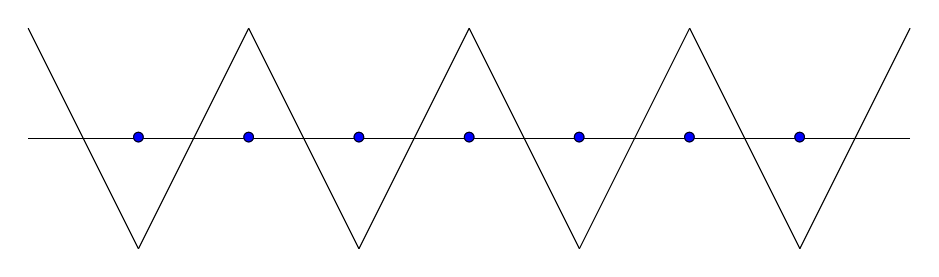
\begin{tikzpicture}[scale=1.4]
	\draw (-4,1) -- (-3,-1) ;
	\draw (-3,-1) -- (-2,1) ;
	\draw (-2,1) -- (-1,-1) ;
	\draw (-1,-1) -- (0,1) ;
	\draw (0,1) -- (1,-1) ;
	\draw (1,-1) -- (2,1) ;
	\draw (2,1) -- (3,-1) ;
	\draw (3,-1) -- (4,1) ;
	
	\draw (4,0) -- (-4,0) ;
	\foreach \k in {-3,...,3}
		{\draw  (\k,0) node[color=blue] {$\bullet$} ;
	   	\draw (\k,0) node {$\circ$} ;
	   	}
\end{tikzpicture}
\end{center}
\caption{Ondes de type "+1/-1".}
\label{fig:hf_waves}
\end{figure}


En considérant cette fonction de grille, on cherche $(a_k)_{0\leq k \leq F}$ tels que $\mathcal{F} \mathfrak{u} = \mathfrak{0}$, soit :
\begin{equation}
\mathcal{F}\mathfrak{u}_i = \gsum_{k=0}^F a_k \dfrac{\mathfrak{u}_{i+k} + \mathfrak{u}_{i-k}}{2} = \gsum_{k=0}^F a_k  \dfrac{(-1)^{i+k} + (-1)^{i-k}}{2} = 0.
\end{equation}
Cette équation est équivalente à 
\begin{equation}
\gsum_{k=0}^F a_k (-1)^k = 0
\label{eq:ftr_ftrcond}
\end{equation}
La relation \eqref{eq:ftr_ftrcond} nous donne une condition alors qu'il y a $F+1$ paramètres à déterminer. Il reste $F$ degrés de libertés dans l'opérateur de filtrage. Le choix qui est fait est de maximiser l'ordre du filtrage de manière à perturber un minimum la donnée initiale tout en supprimant les ondes parasites.

Le filtre doit conserver les très basses fréquences, lorsque $\mathfrak{u} = \mathfrak{1}$, on doit alors $\mathcal{F}\mathfrak{u} = \mathfrak{1}$.
C'est à dire que les coefficients $(a_k)_{0 \leq k \leq F}$ vérifient la relation de consistance
\begin{equation}
\gsum_{k=0}^F a_k = 1
\label{eq:ftr_conscond}
\end{equation}

Enfin, on remarque que si $u : x \in \Omega \mapsto u(x) \in \mathbb{R}$ et si $u^*$ est la fonction de grille associée à $u$, alors on a 
\begin{equation}
\begin{array}{rcl}
u(x_i + kh) & = & u(x_i) + p k u'(x_j) + \cdots + \dfrac{(kh)^l}{l!}u^{(l)}(x_i) + \cdots +\dfrac{(kh)^{2F}}{2F!} u^{(2F)}(\xi_k)\\
u(x_i - kh) & = & u(x_i) - p k u'(x_j) + \cdots + \dfrac{(-kh)^l}{l!}u^{(l)}(x_i) + \cdots +\dfrac{(-kh)^{2F}}{2F!} u^{(2F)}(\eta_k)
\end{array}
\end{equation}
avec $\xi_k \in [x_i, x_i+kh]$ et $\eta_k \in [x_i-kh, x_i]$. Alors par combinaison linéaire en considérant \eqref{eq:ftr_conscond} vérifiée, 
\begin{equation}
\mathcal{F}u^* - u^* = \gsum_{l=1}^{2F-1} \gsum_{k=0}^F \dfrac{a_k}{2} \underbrace{\dfrac{(kh)^l + (-kh)^l}{l!}}_{=0 \text{ pour } l \text{ impair.}}u^{(l)}(x_i) + \gsum_{k=0}^F \dfrac{a_k}{2}\dfrac{(kh)^{2F}}{2F!} \left( u^{(2F)}(\xi_k) + u^{(2F)}(\eta_k) \right)
\end{equation}
Ainsi, la condition de précision est 
\begin{equation}
\gsum_{k=0}^F a_k k^{2l} = 0 \text{ pour } 1 \leq l \leq F-1.
\label{eq:ftr_prescond}
\end{equation}

\begin{theoreme}
Soit $F \in \mathbb{N}^{\star}$. Il existe un unique $(a_k)_{0 \leq k \leq F}$ tel que $\mathcal{F}$ soit à la fois consistant en vérifiant \eqref{eq:ftr_conscond}, précis en vérifiant \eqref{eq:ftr_prescond} et soit un filtre passe bas en satisfesant \eqref{eq:ftr_ftrcond}. L'erreur de troncature du filtre est alors donnée par 
\begin{equation}
\mathcal{F}u^* - u^* = h^{2F} \gsum_{k=0}^F \dfrac{a_k}{2} \dfrac{k^{2F}}{2F!} \left( u^{(2F)}(\xi_k) + u^{(2F)}(\eta_k) \right).
\end{equation}
\label{prop:filter_def}
\end{theoreme}

\begin{proof}
La forme de l'erreur de troncature a déjà été vue, il reste à prouver l'unicité.

Après avoir retiré \eqref{eq:ftr_ftrcond} à \eqref{eq:ftr_conscond}, dire qu'il existe une unique $(a_j)_{0 \leq j \leq J}$ satisfesant les conditions est équivalent à dire que la matrice

\begin{equation}
A=\begin{bmatrix}
1 &  1  &  1  &  1  &  1  &  1  & \cdots\\  
0 &  2  &  0  &  2  &  0  & 2  & \cdots\\
0 &  1  & 2^2 & 3^2 & 4^2 & 5^2 & \cdots\\
0 &  1  & 2^4 & 3^4 & 4^4 & 5^4 & \cdots\\
0 &  1  & 2^6 & 3^6 & 4^6 & 5^6 & \cdots\\
&&& \vdots &  \vdots &
\end{bmatrix} \in \mathbb{M}_{J+1} \left( \mathbb{R} \right)
\end{equation}
est inversible car $a = [a_0, a_1, \cdots, a_J]^T$ est solution de 
\begin{equation}
A a = e_1
\end{equation}
avec $e = [1,1/2, 0,\cdots,0]^T$. En développant la seconde ligne de $A$, on a
\begin{equation}
\det ( A ) = \begin{vmatrix} 
2  &  0  &  2  &  0  & 2  & \cdots\\
1  & 2^2 & 3^2 & 4^2 & 5^2 & \cdots\\
1  & 2^4 & 3^4 & 4^4 & 5^4 & \cdots\\
1  & 2^6 & 3^6 & 4^6 & 5^6 & \cdots\\
& & \vdots &  \vdots &
\end{vmatrix} = 2 \sum_{k=1}^{\lfloor\frac{F-1}{2}\rfloor} \Delta_{2k+1}
\end{equation}
avec $\Delta_k$ donné par
\begin{equation}
\Delta_k = \begin{vmatrix} 
1 & 2^2 & \cdots & (k-1)^2 & (k+1)^2 & \cdots\\
1 & 2^4 & \cdots & (k-1)^4 & (k+1)^4 & \cdots\\
1 & 2^6 & \cdots & (k-1)^6 & (k+1)^6 & \cdots\\
&&& \vdots &  \vdots &
\end{vmatrix} = \dfrac{((F-1)!)^2}{k^2} \begin{vmatrix} 
1 & 1 & \cdots & 1 & 1 & \cdots\\
1 & (2^2)^1 & \cdots & ((k-1)^2)^1 & ((k+1)^2)^1 & \cdots\\
1 & (2^2)^2 & \cdots & ((k-1)^2)^2 & ((k+1)^2)^2 & \cdots\\
&&& \vdots &  \vdots &
\end{vmatrix}
\end{equation}
On reconnaît un déterminant de Van-Der-Monde, donc $\Delta_k = \prod_{1 \leq i < j \leq F-1} \left( \alpha_j - \alpha_i \right)$, avec 
\begin{equation}
\alpha_j = \left\lbrace
\begin{array}{ll}
j^2 & \text{ avec } 1 \leq j \leq k-1\\
(j+1)^2 & \text{ avec } k \leq j \leq J-2\\
\end{array}
\right.
\end{equation}
Si $i<j$, on a $\alpha_i < \alpha_j$, donc $\Delta_k>0$ et $\det A$ est une somme de déterminants tous strictements positifs donc $\det A > 0$. $A$ est inversible et le résultat est prouvé.
\end{proof}
Quelques filtres particuliers sont donnés dans la table \ref{tab:filter} en fonction de leur ordre de précision.
\begin{table}[htbp]
\begin{center}
\begin{tabular}{|c||cccccc|}
\hline
\textbf{Ordre de précision} & $a_0$ & $a_1$ & $a_2$ & $a_3$ & $a_4$ & $a_5$ \\
\hline \hline
$2$ & $1/2$ & $1/2$ & & & & \\
\hline
$4$ & $10/16$ & $8/16$ & $-2/16$ & & & \\
\hline
$6$ & $44/64$ & $30/64$ & $-12/64$ & $2/64$ & & \\
\hline
$8$ & $186/256$ & $112/256$ & $-56/256$ & $16/256$ & $-2/256$ & \\
\hline
$10$ & $772/1024$ & $420/1024$ & $-240/1024$ & $90/1024$ & $-20/1024$ & $2/1024$ \\
\hline
\end{tabular}
\end{center}
\caption{Exemples de filtres de la forme \eqref{eq:ftr} et leurs ordres de précision.}
\label{tab:filter}
\end{table}
Dans la suite, nous supposerons que $(a_k)_{0 \leq k \leq F}$ satisfait les conditions \eqref{eq:ftr_conscond}, \eqref{eq:ftr_prescond} et \eqref{eq:ftr_ftrcond}.
Les valeurs propres et fonctions propres de $\mathcal{F}$ sont issues de la proposition \ref{prop:eigen_P(tau)}.

\begin{theoreme}
Les valeurs propres de $\mathcal{F}$ sont données par $\beta^k$ avec 
\begin{equation}
\beta^k = \gsum_{f=0}^F a_k \cos \left( \dfrac{2 \pi k f}{N} \right)
\end{equation}
pour tout $0 \leq k \leq N-1$, $\beta^k$ est associé à la fonction propre $\mathfrak{u}^k$ telle que 
\begin{equation}
\mathfrak{u}^k_j = \exp \left[ i j \dfrac{2 \pi k}{N} \right].
\end{equation}
\end{theoreme}

On définit le \textit{symbole} du filtre $\mathcal{F}$ par la fonction $\beta : \theta \in [0, \pi] \mapsto \beta(\theta) \in \mathbb{R}$ donnée par :
\begin{equation}
\beta( \theta ) = \gsum_{f=0}^F a_k \cos \left( f \theta \right)
\end{equation}

\begin{proposition}
Il existe un unique polynôme $P$ de degré $F$ tel que 
\begin{equation}
\beta(\theta) = P(\cos \theta )
\end{equation}
De plus,
\begin{equation}
P(x) = 1 -\dfrac{1}{(-2)^F} (X - 1)^F.
\end{equation}
\end{proposition}

\begin{proof}
Soit $\theta \in [0, \pi]$, 
\begin{equation}
\beta(\theta) = \gsum_{f=0}^F a_f \cos \left( f \theta \right) = \gsum_{f=0}^F a_f T_f ( \cos \theta )
\end{equation}
où $T_f \in \mathbb{R}_f [X]$ est le $k-$ieme polynome de Tchebytchev. 
Ainsi il existe $P \in \mathbb{R}_F [x]$ tel que $\beta( \theta ) = P( \cos \theta )$. Ce polynôme est unique. Montrons que 
\begin{equation}
P(x) = 1 -\dfrac{1}{(-2)^F} (X - 1)^F.
\end{equation}
convient.

\begin{itemize}
\item on montre facilement que 
\begin{equation}
P( \cos 0 ) = 1 -\dfrac{1}{(-2)^F} (\cos 0 - 1)^F = 1,
\end{equation}
de même,
\begin{equation}
P( \cos \pi ) = 1 -\dfrac{1}{(-2)^F} (\cos \pi - 1)^F 1 -\dfrac{(-2)^F}{(-2)^F} = 0.
\end{equation}
\item On rappelle la formule de Fàa Di Bruno permettant de calculer la dérivée $n-$ième d'une composée. Si $f$ et $g$ sont des fonctions régulières, on a 
\begin{equation}
\dfrac{d^n}{dx^n} \left( f \circ g \right)(x) = \gsum_{k=1}^n f^{(k)}\left( g(x) \right) B_{n,k}\left( g'(x), g''(x), \cdots , g^{n-k+1}(x) \right)
\end{equation}
où $B_{n,k}$ est un polynôme de Bell. En utilisant cette formule avec $f = P$ et $g = \cos$, évaluée en $\theta = 0$, on montre que :
\begin{equation}
\dfrac{d^n}{d\theta^n} \left( P \circ \cos \right)(0) = \gsum_{k=1}^n P^{(k)}\left(1\right) B_{n,k}\left( -1,0,1,0, \cdots\right)
\end{equation}
Or, $P^{(k)}\left(1\right) = 0$ pour tout $k \geq 1$. Donc 
\begin{equation}
\dfrac{d^n}{d\theta^n} \left( P \circ \cos \right)(0) = 0
\end{equation}
\end{itemize}
Le polynôme $P$ convient et 
\begin{equation}
\beta( \theta ) = 1 - \dfrac{1}{(-2)^F}(\cos \theta -1)^F.
\end{equation}
\end{proof}

\begin{proposition}
Pour tout $\theta \in [0, \pi]$, on a 
\begin{equation}
0 \leq \beta ( \theta ) \leq 1
\end{equation}
\end{proposition}

\begin{proof}
Supposons qu'il existe $\theta \in [0, \pi]$ tel que $\beta(\theta) < 0$ ou $\beta(\theta) > 1$. Comme $\beta(0)=1$ et $\beta(\pi) = 0$, il existe $\tilde{\theta} \in ]0, \pi[$ tel que 
\begin{equation}
\beta'(\tilde{\theta}) = - \sin \tilde{\theta} P'(\cos \tilde{\theta} ) = 0
\end{equation}
Or $\sin \tilde{\theta} \neq 0$ pour $\tilde{\theta} \in ]0, \pi[$.
De plus, 
\begin{equation}
P'(X) = \dfrac{F}{(-2)^F}(X-1)^{F-1}
\end{equation}
donc en prenant $X = \cos \tilde{\theta}$,
\begin{equation*}
P'(X) = 0 \Leftrightarrow \cos \tilde{\theta} = 1
\end{equation*}
Ce qui est impossible pour $\tilde{\theta} \in ]0, \pi[$. Donc par l'absurde, le résultat est vérifié.
\end{proof}

La fonction $\beta$ permet de considérer le comportement du filtre sur les différentes fréquences $\theta \in [0, \pi]$. Les basses fréquences sont bien conservées alors que les hautes fréquences ($\theta$ proche de $\pi$) sont atténuées. Cette observation est visible sur la figure \ref{fig:freq_filter} représentant la fonction $\beta : \theta \mapsto \beta(\theta)$ associée aux filtres d'ordre 2, 4, 6, 8 et 10. 

\begin{figure}[htbp]
\begin{center}
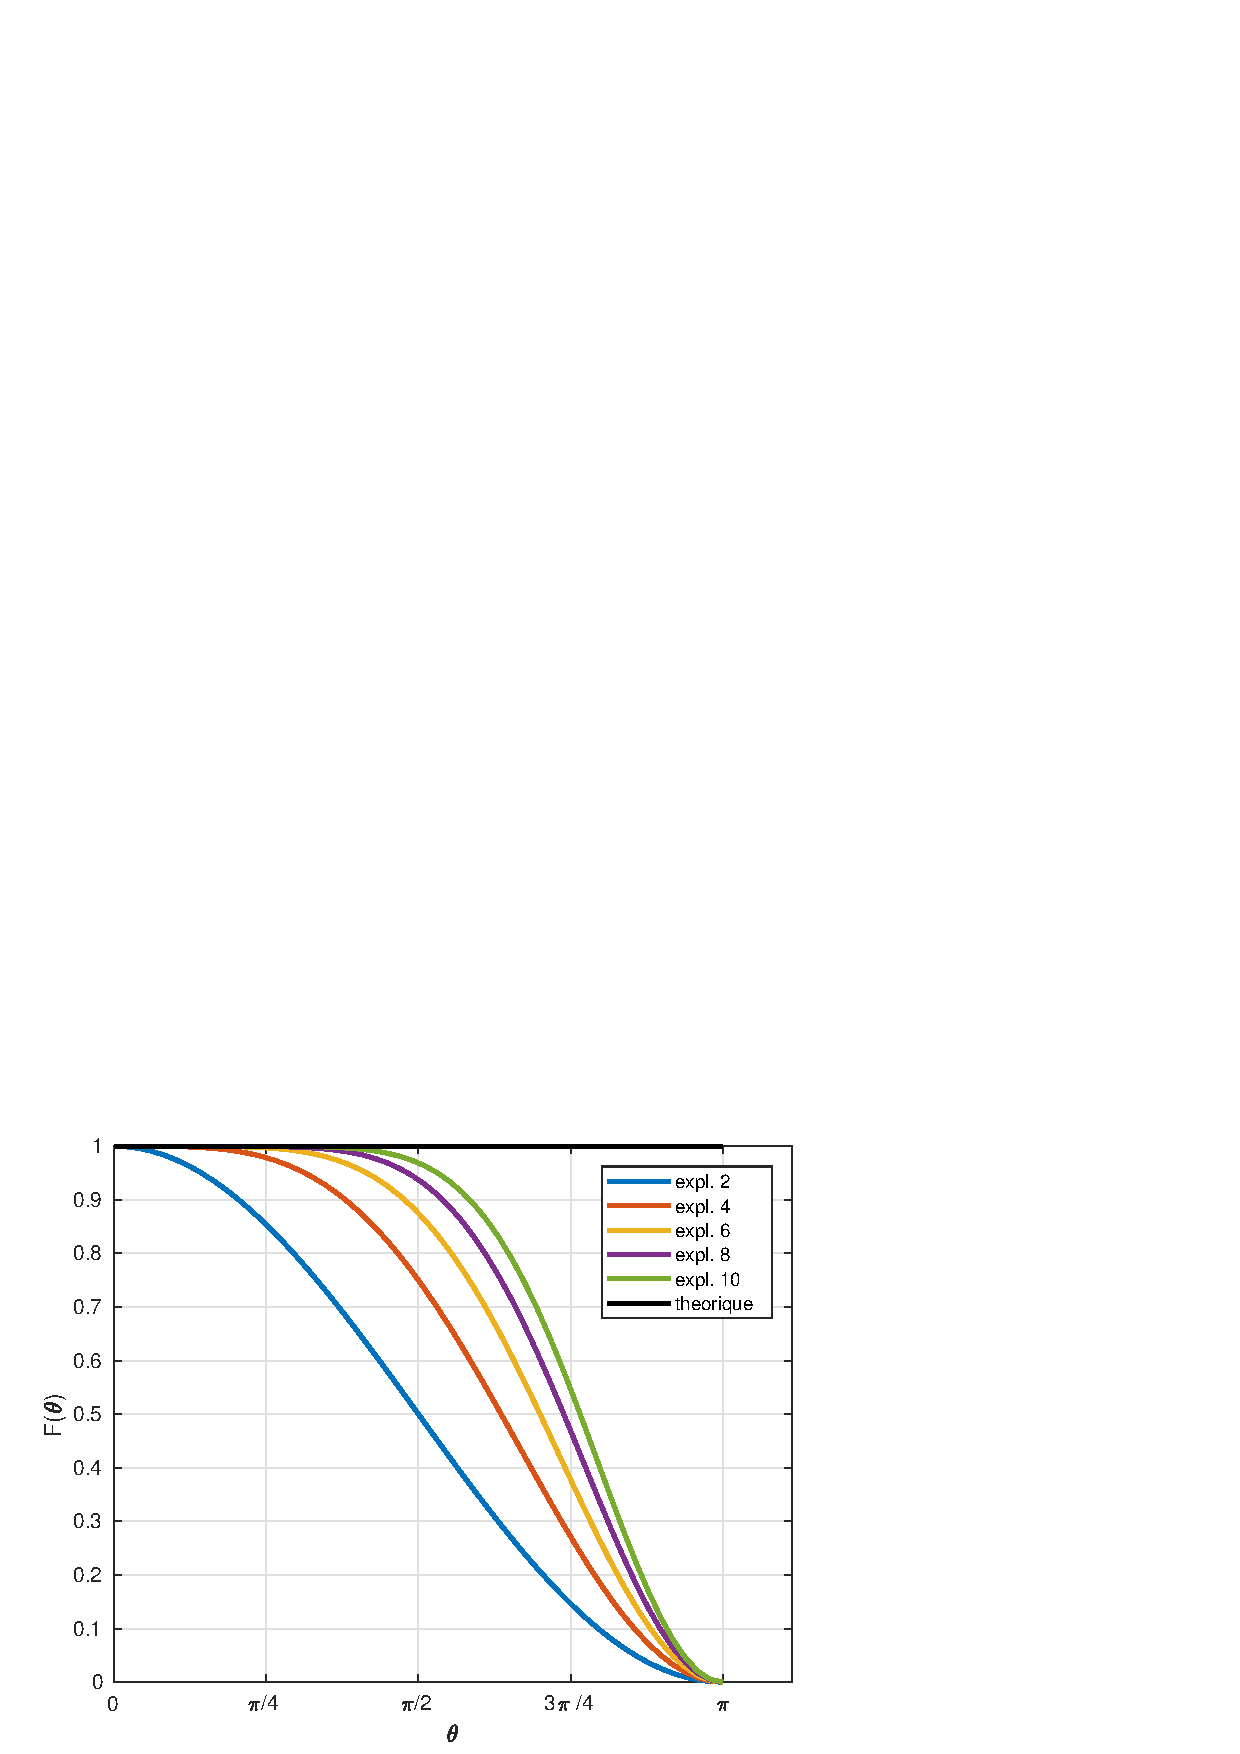
\includegraphics[scale=0.7]{freq_filter.png}
\end{center}
\caption{Fonction d'amplification $\beta$ pour les filtres explicites d'ordre 2, 4, 6, 8 et 10.}
\label{fig:freq_filter}
\end{figure}
Comme on s'y attendais, un filtre d'ordre élevé laisse passer un plus grand nombre de basses fréquences. Dans le tableau \ref{tab:filter_095}, on représente la fréquence $\theta_{0.95}$ maximale qui est conservée à $95\%$. Comme la fonction $\beta$ est strictement décroissante et continue sur $[0,\pi]$, c'est une bijection de $[0,\pi]$ dans $[0,1]$ et on a 
\begin{equation}
\theta_{0.95} = \beta^{-1}(0.95)= \arccos \left[ 1-2 (0.05)^{1/F} \right].
\end{equation}

\begin{table}
\begin{center}
\begin{tabular}{|c||c|}
\hline
\textbf{Ordre du filtre} & \textbf{Fréquence conservée à } $95\%$\\
\hline
\hline
$10$&$1.6695$\\
$8$&$1.5165$\\
$6$&$1.3045$\\
$4$&$0.9851$\\
$2$&$0.4510$\\
\hline
\end{tabular}
\end{center}
\caption{Fréquence conservée à $95\%$ en fonction de l'ordre du filtre.}
\label{tab:filter_095}
\end{table}

La fonction $F \mapsto \theta_{0.95} = \beta^{-1}(0.95)$ est croissante, ce qui confirme que lorsque l'ordre de précision croit, $\theta_{0.95}$ croit et le filtre conserve un plus grand nombre de fréquences. De plus, 
\begin{equation}
\lim_{F \rightarrow +\infty} \theta_{0.95} = \pi.
\end{equation}
Ce qui confirme la prise en compte d'un grand nombre de fréquence lorsque l'on augmente l'ordre du filtre. Cependant lorsque l'ordre du filtre augmente, l'effet de filtrage des hautes fréquences diminue.

Le filtre utilisé est linéaire et agit sur les composantes des fonctions de grilles. Si $\mathfrak{u}$ est une fonction de grille, on pose $U$ et $\tilde{U}$ les vecteurs de $\mathbb{R}^N$ tel que
\begin{equation}
U = \begin{bmatrix}
\mathfrak{u}_1\\
\mathfrak{u}_2\\
\vdots \\
\mathfrak{u}_N\\
\end{bmatrix} \text{ et } 
\tilde{U} = \begin{bmatrix}
\mathcal{F}\mathfrak{u}_1\\
\mathcal{F}\mathfrak{u}_2\\
\vdots \\
\mathcal{F}\mathfrak{u}_N\\
\end{bmatrix}
\end{equation}
Alors $U$ et $\tilde{U}$ vérifient la relation
\begin{equation}
\tilde{U} = M U
\end{equation}
avec $M \in \mathbb{M}_N \left( \mathbb{R} \right)$ la matrice associée au filtrage des données en dimension 1. Lorsque le filtre est d'ordre 4, ($F=2$), la matrice $M$ est donnée par
\begin{equation}
M = \dfrac{1}{2}
\begin{bmatrix}
2a_0 & a_1 & a_2 &   &   &   & a_2 & a_1 \\ 
a_1 & 2 a_0 & a_1 & a_2 &   &   &   & a_2 \\ 
a_2 & a_1 & 2a_0 & a_1 & a_2 & (0) &   &   \\ 
  & a_2 & a_1 & 2a_0 & a_1 & a_2 &   &   \\ 
  &   & \ddots & \ddots & \ddots & \ddots & \ddots &   \\ 
  &   & (0) & a_2 & a_1 & 2 a_0 & a_1 & a_2 \\ 
a_2 &   &   &   & a_2 & a_1 & 2a_0 & a_1 \\ 
a_1 & a_2 &   &   &   & a_2 & a_1 & 2a_0
\end{bmatrix}
\end{equation}
Plus généralement, pour un filtre d'ordre quelconque, on a
\begin{equation}
M_{i,j} = \left\lbrace
\begin{array}{cl}
a_0 & \text{ si } i=j \\
\dfrac{1}{2} a_k & \text{ si } i+j \equiv k [N]\\
0 & \text{ sinon.}
\end{array}
\right.
\end{equation}
La matrice $M$ est symétrique.




































\section{Opérateurs aux différences en dimension 2}


\subsection{Notations}
\label{sec:notation_2D}

En dimension 2, les notations sont analogues de celles utilisées en dimension 1. On se limite au cas d'une géométrie carrée. Si $a$ et $b$ sont des réels positifs, nous notons $\Omega = [a,b]^2$. Chaque côté du carré est de longueur $L=b-a$. 
Soient $u$ et $v$ deux fonctions de $\Omega$ dans $\mathbb{R}$. On note le produit scalaire dans $L^2 ( \Omega )$
\begin{equation}
(u,v) = \gint_{\Omega} u(x,y) v(x,y) dx dy.
\end{equation}
La norme associée est :
\begin{equation}
\| u \|_{L^2(\Omega)} = \sqrt{(u,v)}. 
\end{equation}
On note également
\begin{equation}
\| u \|_{L^{\infty} ( \Omega )} = \max_{(x,y) \in \Omega} |u(x,y)|.
\end{equation}
Pour alléger les notations nous notons ces deux normes $\| u \|_{L^2}$ et $\| u \|_{L^{\infty}}$.

Dans le domaine $\Omega$, la grille est constituée des points $(x_i,y_j)_{0 \leq i,j \leq N}$ où $N \geq 1$ avec $a = x_0 < x_1 < \ldots < x_N = b$ et $a = y_0 < y_1 < \ldots < y_N = b$. Le pas d'espace $h$ est fixe et donné par $h = \frac{L}{N}$. Les points de grilles sont $(x_i, y_j)$ avec 
\begin{equation}
\left\lbrace\begin{array}{rcl}
x_i & = & a + i h \\
y_j & = & a + j h 
\end{array}\right. \text{ avec } 0 \leq i,j \leq N.
\end{equation}

Les points $(x_i,y_j)_{0 \leq i,j \leq N}$ sont de deux types (voir figure \ref{fig:maillage2D}) :
\begin{itemize}
\item Les points de bords $(x_i, y_j)$ avec
\begin{equation}
i \in \left\lbrace 0 , N \right\rbrace \text{ ou } j \in \left\lbrace 0 , N \right\rbrace,
\end{equation}
\item les points intérieurs $(x_i, y_j)$ avec
\begin{equation}
1 \leq i,j \leq N-1.
\end{equation}
\end{itemize}



\begin{figure}[htbp]
\begin{center}
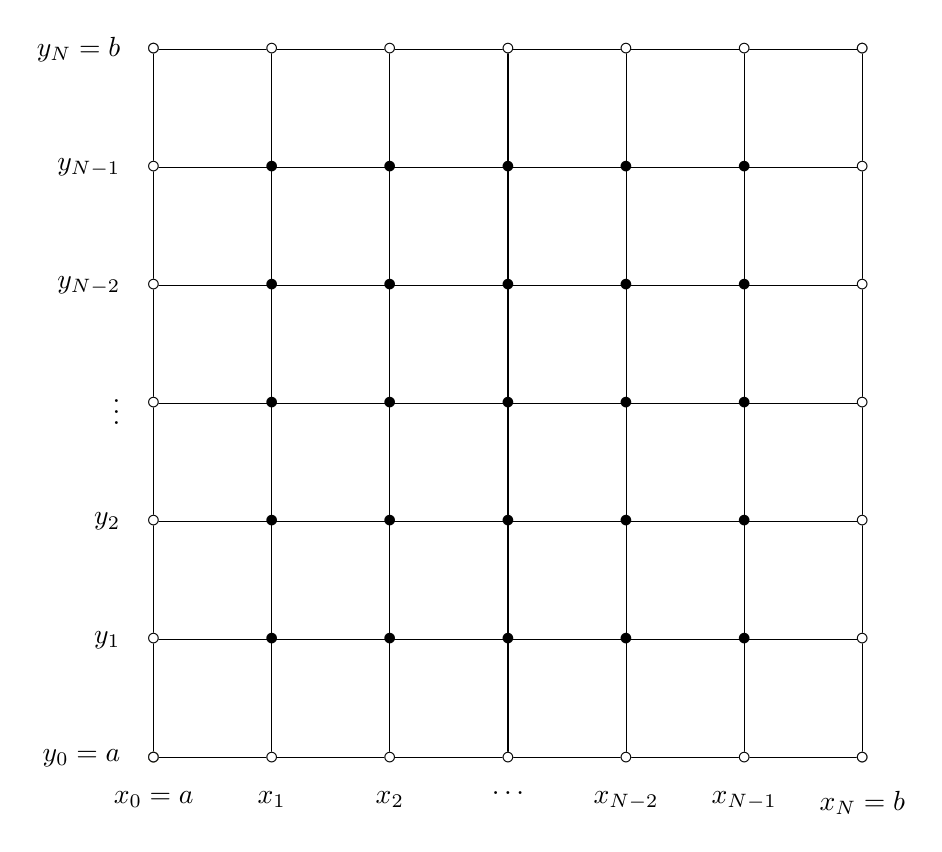
\begin{tikzpicture}[scale=1.5]
	\draw (-3,-3.2) node[below] {$x_0=a$} ;
	\draw (-2,-3.2) node[below] {$x_1$} ;
	\draw (-1,-3.2) node[below] {$x_2$} ;
	\draw (0,-3.2) node[below] {$\ldots$} ;
	\draw (1,-3.2) node[below] {$x_{N-2}$} ;
	\draw (2,-3.2) node[below] {$x_{N-1}$} ;
	\draw (3,-3.2) node[below] {$x_N =b$} ;
	
	\draw (-3.2,-3) node[left] {$y_0=a$} ;
	\draw (-3.2,-2) node[left] {$y_1$} ;
	\draw (-3.2,-1) node[left] {$y_2$} ;
	\draw (-3.2,0) node[left] {$\vdots$} ;
	\draw (-3.2,1) node[left] {$y_{N-2}$} ;
	\draw (-3.2,2) node[left] {$y_{N-1}$} ;
	\draw (-3.2,3) node[left] {$y_N =b$} ;
	
	\draw (-3,-3) grid[step=1] (3,3);

	\draw (-3,-3) node[color=yellow] {$\bullet$} ;
	\draw (-3,-3) node {$\circ$} ;
	
	\foreach \k in {-3,...,3}
		{\draw  (\k,-3) node[color=white] {$\bullet$} ;
	   	\draw (\k,-3) node {$\circ$} ;
	   	\draw  (\k,3) node[color=white] {$\bullet$} ;
	   	\draw (\k,3) node {$\circ$} ;
	   	\draw  (-3,\k) node[color=white] {$\bullet$} ;
	   	\draw (-3,\k) node {$\circ$} ;
	   	\draw  (3,\k) node[color=white] {$\bullet$} ;
	   	\draw (3,\k) node {$\circ$} ;
	   	}
	   	
	\foreach \k in {-2,...,2}
		{\draw  (\k,-2) node {$\bullet$};
		\draw  (\k,-1) node {$\bullet$};
		\draw  (\k,0) node {$\bullet$};
		\draw  (\k,1) node {$\bullet$};
		\draw  (\k,2) node {$\bullet$};
	   	}
\end{tikzpicture}
\end{center}
\caption{Grille en dimension 2. Les symboles $\circ$ désignent les points de bords, les symboles $\bullet$ désignent les points intérieurs de la grille.}
\label{fig:maillage2D}
\end{figure}

On dit qu'une fonction $u : (x,y) \in \mathbb{R} \mapsto u(x,y) \in \mathbb{R}$ est $L-$\textit{périodique} dans les directions $x$ et $y$ si 
\begin{equation}
\begin{array}{rcl}
u(x,y+L) & = & u(x,y) \\
u(x+L,y) & = & u(x,y)
\end{array} \text{ pour tous } (x,y) \in \mathbb{R}^2.
\end{equation}

Comme en dimension 1, nous définissons différentes notions de fonctions discrètes associées à la grille :
\begin{enumerate}
\item Une \textit{fonction de grille} est une fonction définie aux points de la grille $(x_i,y_j)_{0 \leq i,j \leq N}$. Nous notons ces fonctions en fonte gothique comme $\mathfrak{u}$ ou $\mathfrak{v}$. On a :
\begin{equation}
\mathfrak{u} = \left( \mathfrak{u}(x_i,y_j) \right)_{0 \leq i,j \leq N} \text{ et } \mathfrak{u}_{i,j} = \mathfrak{u}(x_i,y_j).
\end{equation}
$\mathfrak{u}$ est périodique si $\mathfrak{u}(x_{i},y_0) = \mathfrak{u}(x_{i},y_N)$ et $\mathfrak{u}(x_{0},y_j) = \mathfrak{u}(x_{N},y_j)$ pour tous $0 \leq i,j \leq N$.
On note $L^2_h$ l'espace des fonctions de grilles. Cet espace est équipé d'un produit scalaire et de la norme associée :
\begin{equation}
(\mathfrak{u}, \mathfrak{v})_h = h^2 \gsum_{i,j=0}^N \mathfrak{u}(x_i,y_j) \mathfrak{v}(x_i,y_j) \text{ et } |\mathfrak{u}|_h = \sqrt{(\mathfrak{u},\mathfrak{u})_h}.
\end{equation}
de plus, on a également
\begin{equation}
| \mathfrak{u} |_{\infty} = \max_{0 \leq i,j \leq N} |\mathfrak{u}(x_i,y_j)|.
\end{equation}
Pour simplifier les notations, nous noterons
\begin{equation}
\mathfrak{u}_{i,j} = \mathfrak{u}(x_i, y_j) \text{ avec } 1 \leq i,j \leq N.
\end{equation}

\item Soit $u : (x,y) \in \Omega \mapsto u(x,y) \in \mathbb{R}$, nous définissons la fonction associée, notée $u^*$ par la restriction de $u$ à la grille :
\begin{equation}
u^*_{i,j} = u(x_i, y_j) \text{ pour tous } 0 \leq i,j \leq N.
\end{equation}

Pour $u$ est périodique selon $x$ et $y$, on a $u^*_{i,0}=u^*_{i,N}$ et $u^*_{0,j}=u^*_{N,j}$ pour tous $0 \leq i,j \leq N$.
D'une manière générale, dans un contexte périodique, les données sur des bords opposés du carrés coïncident.

\item A une fonction de grille $\mathfrak{u}$, on associe un vecteur $U \in \mathbb{R}^{(N+1)^2}$ constitué des valeurs de $\mathfrak{u}$ dans l'ordre anti-lexicographique :
\begin{equation}
U = \begin{bmatrix}
\mathfrak{u}_{0,0}\\
\mathfrak{u}_{1,0}\\
\vdots \\
\mathfrak{u}_{N,0}\\
\mathfrak{u}_{0,1}\\
\mathfrak{u}_{1,1}\\
\vdots \\
\mathfrak{u}_{N,1}\\
\vdots \\
\mathfrak{u}_{N,N}\\
\end{bmatrix}.
\end{equation}
On note ces vecteurs par des lettres capitales. Les matrices de $\mathbb{M}_{(N+1)^2} (\mathbb{R})$, notée par des lettres latines capitales, agissent sur ces vecteurs.
\end{enumerate}

\begin{figure}[htbp]
\begin{center}
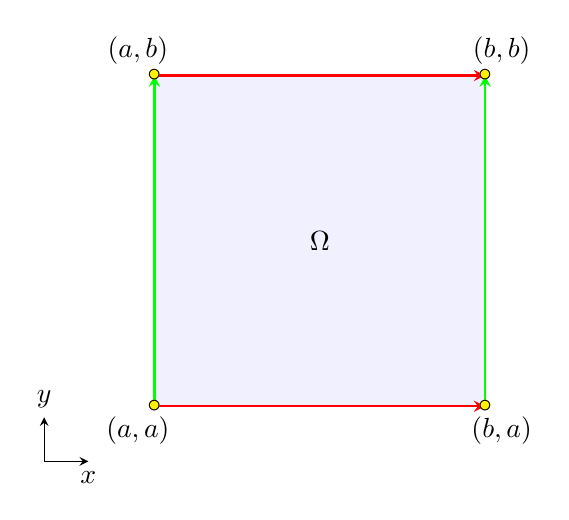
\begin{tikzpicture}[scale=.7]
	\filldraw[draw=black,fill=blue!30!white,opacity=0.20]
	plot (-3,-3) -- (-3,3)
	-- plot (-3,3) -- (3,3)
	-- plot (3,3) -- (3,-3)
	-- plot (3,-3) -- (-3,-3)
	-- cycle;

	\draw [>=stealth, ->,color=green,thick] (-3,-3) -- (-3,3) ;
	\draw [>=stealth, ->,color=green,thick] (3,-3) -- (3,3) ;
	\draw [>=stealth, ->,color=red,thick] (-3,-3) -- (3,-3) ;
	\draw [>=stealth, ->,color=red,thick] (-3,3) -- (3,3) ;
	
	\draw (-3.3,-3.45) node {$(a,a)$} ;
	\draw (3.3,-3.45) node {$(b,a)$} ;
	\draw (-3.3,3.45) node {$(a,b)$} ;
	\draw (3.3,3.45) node {$(b,b)$} ;
	\draw (0,0) node {$\Omega$} ;
	\draw  (-3,-3) node[color=yellow] {$\bullet$} ;
	\draw (-3,-3) node {$\circ$} ;
	\draw  (3,-3) node[color=yellow] {$\bullet$} ;
	\draw (3,-3) node {$\circ$} ;
	\draw  (-3,3) node[color=yellow] {$\bullet$} ;
	\draw (-3,3) node {$\circ$} ;
	\draw  (3,3) node[color=yellow] {$\bullet$} ;
	\draw (3,3) node {$\circ$} ;
	\draw [>=stealth, ->] (-5,-4) -- (-4.2,-4) ;
	\draw (-4.2,-4) node[below] {$x$} ;
	\draw [>=stealth, ->] (-5,-4) -- (-5,-3.2) ;
	\draw (-5,-3.2) node[above] {$y$} ;
\end{tikzpicture}
\end{center}
\caption{Carré périodique. Dans le contexte périodique, les données sur les bords de couleurs identiques coïncident. Les quatre coins du carré représentent la même donnée.}
\label{fig:period2D}
\end{figure}
























\subsection{Opérateurs en géométrie cartésienne}

En utilisant les notations de la partie \ref{sec:notation_2D} en contexte périodique, nous définissons des opérateurs agissant sur les fonctions de grilles en dimension 2.

\begin{definition}
Soient $\tau_x$ et $\tau_y$ les \textit{opérateurs de translation} dans les directions $x$ et $y$ définis par
\begin{equation}
\left\lbrace
\begin{array}{rcl}
\tau_x \mathfrak{u}_{i,j} & = & \mathfrak{u}_{i+1,j}\\
\tau_y \mathfrak{u}_{i,j} & = & \mathfrak{u}_{i,j+1}\\
\end{array}
\right.
\end{equation}
avec $\mathfrak{u}$ une fonction de grille et $1 \leq i,j \leq N$.
\end{definition}

Les opérateurs obtenus en dimension 1 sont définis en dimension 2 grâce à ces deux opérateurs de translation. On définit les opérateurs centrés dans les directions $x$ et $y$ par 
\begin{equation}
\left\lbrace
\begin{array}{rcl}
\delta_x & = & \dfrac{\tau_x - \tau_x^{-1}}{2h} \\
\delta_y & = & \dfrac{\tau_y - \tau_y^{-1}}{2h}
\end{array}
\right.
\label{eq:der_centrée_2D}
\end{equation}
De la même manière, on définis les opérateurs de Simpson dans chaque direction par 
\begin{equation}
\left\lbrace
\begin{array}{rcl}
\sigma_x & = & \dfrac{1}{6} \tau_x + \dfrac{4}{6} id + \dfrac{1}{6} \tau_x^{-1} \\
\sigma_y & = & \dfrac{1}{6} \tau_y + \dfrac{4}{6} id + \dfrac{1}{6} \tau_y^{-1} \\
\end{array}
\right.
\label{eq:simpson_2D}
\end{equation}
Chacun des opérateurs $\sigma_x$ et $\sigma_y$ est inversible.
L'opérateur hermitien en dimension 1 $\delta_x^H$ est étendue en dimension 2 grâce à la relation suivante 
\begin{equation}
\left\lbrace
\begin{array}{rcl}
\delta_x^H & = & \sigma_x^{-1} \circ \delta_x \\
\delta_y^H & = & \sigma_y^{-1} \circ \delta_y
\end{array}
\right.
\label{eq:der_herm_2D}
\end{equation}

\begin{theoreme}
Soit $u : x \in \Omega \mapsto u(x) \in \mathbb{R}$ est une fonction de $\mathcal{C}^5 (\Omega)$. On note $u^*$ la fonction de grille associée à $u$ et $u_x^*$ (resp. $u_y^*$) la fonction de grille associée à la dérivée de $u$ dans la direction $x$ (resp. $y$) notée $\partial_x u$ (resp. $\partial_y u$). Alors
\begin{equation}
\begin{array}{rcl}
|u^*_{x} - \delta_x^H u^*|_{\infty} &\leq& C h^4\\
|u^*_{y} - \delta_y^H u^*|_{\infty} &\leq& C h^4
\end{array}
\end{equation}
\end{theoreme}

\begin{proof}
Conséquence du théorème \ref{prop:consistence_herm2} appliqué dans chaque direction $x$ et $y$.
\end{proof}













\subsection{Écriture matricielle des opérateurs}

Dans cette section, nous précisons les notations vectorielles et matricielles utiles à l'écriture matricielle des opérateurs en dimension 2.

Nous définissons la \textit{base canonique} de $\mathbb{R}^N$, notée $\left(e_i \right)_{1 \leq i \leq N}$ et donnée par 
\begin{equation}
\left( e_i \right) = \delta_{i,j} = \left\lbrace
\begin{array}{rl}
1 & \text{ si } j=i,\\
0 & \text{ sinon.}
\end{array}
\right.
\end{equation}
$\delta_{i,j}$ est le symbole de Kronecker.

\begin{definition}
Soit $A$ une matrice de taille $m \times n$ et $B$ une matrice de $p \times q$, avec $m, n, p, q \in \mathbb{N}^{\star}$. La matrice $A \otimes B$ est une matrice de taille $mp \times nq$ donnée comme le produit de Kronecker de $A$ par $B$ et 
\begin{equation}
A \otimes B = 
\begin{bmatrix}
a_{1,1}B & \cdots & a_{1,n}B \\ 
\vdots & \ddots & \vdots \\ 
a_{n,1}B & \cdots & a_{n,n}B
\end{bmatrix} 
\end{equation}
\end{definition}
On rapelle les propriétés suivantes concernant le produit de Kronecker :

\begin{proposition}
Soient $A$, $B$, $C$ et $D$ des matrices et $\alpha$ un réel.
\begin{itemize}
\item La multiplication par un scalaire vérifie
\begin{equation}
\alpha ( A \otimes B ) = \alpha A \otimes B = A \otimes \alpha B,
\end{equation}

\item si les produits $AC$ et $BD$ sont bien définis alors
\begin{equation}
(A \otimes B ) (C \otimes D) = AC \otimes BD,
\end{equation} 


\item si $A$ et $B$ sont inversibles
\begin{equation}
(A \otimes B)^{-1} = A^{-1} \otimes B^{-1}.
\end{equation}
\end{itemize}
\label{prop:pdt_kron}
\end{proposition}
L'application $\text{vec}_2$ permet de transformer une fonction de grille $\mathbf{u}$ en un vecteur $U$.

\begin{definition}
L'opérateur $\text{vec}_2$ est défini par
\begin{equation}
\begin{array}{rcl}
\text{vec}_2 : L^2_h & \longrightarrow & \mathbb{R}^{N^2}\\
\mathfrak{v} & \longrightarrow & V = \text{vec}_2(\mathfrak{v})
\end{array}
\end{equation}
avec
\begin{equation}
\text{vec}_2(\mathfrak{v}) = \gsum_{i,j=1}^N \left( e_j \otimes e_i \right)\mathfrak{v}_{i,j}.
\end{equation}
\end{definition}

L'opérateur $\text{vec}_2$ transforme une fonction de grille $\mathfrak{v}$ en un vecteur en organisant les données dans l'ordre antilexicographique. Si $V = \text{vec}_2 (\mathfrak{v})$ alors on a l'égalité suivante :
\begin{equation}
V=[\mathfrak{v}_{1,1}, \mathfrak{v}_{2,1}, \mathfrak{v}_{3,1}, \cdots, \mathfrak{v}_{N,1}, \mathfrak{v}_{1,2}, \mathfrak{v}_{2,2}, \cdots,  \mathfrak{v}_{N-1,N}, \mathfrak{v}_{N,N}]^T
\end{equation}

\begin{proposition}
Soit $\mathfrak{u}$ une fonction de grille. Alors les opérateurs de dérivées centrées \eqref{eq:der_centrée_2D} s'écrivent matriciellement sous la forme
\begin{equation}
\left\lbrace
\begin{array}{rcl}
\text{vec}_2(\delta_x \mathfrak{u}) & = & (Id \otimes K) \text{vec}_2(\mathfrak{u})\\
\text{vec}_2(\delta_y \mathfrak{u}) & = & (K \otimes Id) \text{vec}_2(\mathfrak{u})\\
\text{vec}_2(\sigma_x \mathfrak{u}) & = & (Id \otimes P) \text{vec}_2(\mathfrak{u})\\
\text{vec}_2(\sigma_y \mathfrak{u}) & = & (P \otimes Id) \text{vec}_2(\mathfrak{u})\\
\end{array}\right.
\end{equation}
\label{prop:op_der_simpson_mat}
\end{proposition}

\begin{proof}
Par définition de $\text{vec}_2$, on a 
\begin{align*}
\text{vec}_2 (\delta_x \mathfrak{u}) &= \gsum_{i,j=1}^N (e_j \otimes e_i) \delta_x \mathfrak{u_{i,j}} \\
	&= \dfrac{1}{2h} \gsum_{i,j=1}^N (e_j \otimes e_i) \left( \mathfrak{u}_{i+1,j} - \mathfrak{u}_{i-1,j} \right) \\
	&= \dfrac{1}{2h} \gsum_{i,j=1}^N e_j \otimes e_i \mathfrak{u}_{i+1,j} - e_j \otimes e_i \mathfrak{u}_{i-1,j}\\
	&= \dfrac{1}{2h} \gsum_{i,j=1}^N e_j \otimes (e_i \mathfrak{u}_{i+1,j}-e_i \mathfrak{u}_{i-1,j}) \\
	&= (Id \otimes K) \text{vec}_2(\mathfrak{u}).
\end{align*}
les autres égalités se montrent de la même manière
\end{proof}

De ces égalités, il découle le calcul matriciel de $\delta_x^H \mathfrak{u}$ et de $\delta_y^H \mathfrak{u}$.

\begin{theoreme}
Soit $\mathfrak{u}$ une fonction de grille. Alors, si on pose 
\begin{equation}
\left\lbrace
\begin{array}{rcl}
U & = & \text{vec}_2 (\mathfrak{u}) \\
U_x & = & \text{vec}_2 (\delta_x^H \mathfrak{u}) \\
U_y & = & \text{vec}_2 (\delta_y^H \mathfrak{u}) \\
\end{array}
\right.
\end{equation}
alors les égalités suivantes sont vérifiées
\begin{equation}
\left\lbrace
\begin{array}{rcccl}
U_x &=& (Id \otimes P)^{-1}(Id \otimes K) U &=& (Id \otimes P^{-1}K)U \\
U_y &=& (P \otimes Id)^{-1}(K \otimes Id) U &=& (P^{-1}K \otimes Id)U\\
\end{array}
\right.
\end{equation}
\end{theoreme}

\begin{proof}
Conséquence directe des propositions \ref{prop:op_der_simpson_mat} et \ref{prop:pdt_kron}.
\end{proof}

La matrice du schéma hermitien $(Id \otimes P^{-1}K)$ en direction $x$ et $(P^{-1}K \otimes Id)$ en direction $y$ vérifient des propriétés d'antisymétriques similaires à celles en dimension 1.
\begin{proposition}
Les matrices $(Id \otimes P^{-1}K)$ et $(P^{-1}K \otimes Id)$ sont antisymétrique.
\end{proposition}

\begin{proof}
$P^{-1}K$ est antisymétrique. D'où le résultat.
\end{proof}





















\subsection{Opérateur de filtrage}

Dans cette partie, nous utilisons toujours les notations de la section \ref{sec:notation_2D} en contexte périodique. Définissons les opérateurs de filtrage dans les directions $x$ et $y$ par
\begin{eqnarray*}
\mathcal{F}_x = \gsum_{k=0}^F a_k \dfrac{\tau_x^k + \tau_x^{-k}}{2} \\
\mathcal{F}_y = \gsum_{k=0}^F a_k \dfrac{\tau_y^k + \tau_y^{-k}}{2} \\
\end{eqnarray*}

Avec $(a_k)_{0 \leq k \leq F}$ vérifiant \ref{prop:filter_def}. Comme la géométrie est cartésienne, on remarque que 
\begin{equation}
\mathcal{F}_x \circ \mathcal{F}_y = \mathcal{F}_y \circ \mathcal{F}_x.
\end{equation}
Ce qui est faux lorsque la métrique n'est pas orthogonale.
La proposition \ref{prop:filter_def} permet de vérifier la consistance des opérateurs de filtrages.
Si $u : (x,y) \in \Omega \mapsto u(x,y) \in \mathbb{R}$ est fonction de $\mathcal{C}^{2F}$ alors :
\begin{eqnarray*}
\mathcal{F}_x u^*_{i,j} - u^*_{i,j} & = & C_xh^{2F}\\
\mathcal{F}_y u^*_{i,j} - u^*_{i,j} & = & C_yh^{2F}
\end{eqnarray*}
où $C_x$ et $C_y$ sont des constantes indépendantes de $h$.
En particulier, en composant les opérateurs, on peut définir un nouvel opérateur de filtrage. En effet  
\begin{equation}
(\mathcal{F}_x \circ \mathcal{F}_y) u_{i,j}^* - u_{i,j}^* = Ch^{2F}.
\end{equation}

L'écriture matricielle de l'opérateur de filtrage est donnée par la proposition suivante :
\begin{proposition}
Soit $\mathbf{u}$ une fonction de grille. Alors les opérateurs de filtrages s'écrivent à l'aide de matrices comme :
\begin{equation}
\left\lbrace
\begin{array}{rcl}
\text{vec}_2 (\mathcal{F}_x \mathbf{u}) & = & (Id \otimes M) \text{vec}_2 (\mathbf{u})\\
\text{vec}_2 (\mathcal{F}_y \mathbf{u}) & = & (M \otimes Id) \text{vec}_2 (\mathbf{u})\\
\end{array}
\right.
\end{equation}
\end{proposition}
Comme la matrice $M$ est symétrique, il est immédiat que $Id \otimes M$ et $M \otimes Id$ sont symétriques aussi.

